\noindent\emph{This document accompanies the manuscript and its Supplementary Document (Tables S1--S10, Algorithms S1--S5) and is distributed with the code repository rather than submitted to the journal. Sections, tables, and figures are numbered R1--R12, R1--R23, and R1--R5 (R for repository, to keep them apart from experiments E0--E4).}

\section{Lessons from the Implementation}
\label{app:lessons}
Table~\ref{tab:lessons} details the conditions summarized in Section~\ref{M-sec:discussion} of the main text.

\begin{table*}[h]
\centering
\caption{Conditions that the implementation revealed: the premise of a construct as commonly described, what we observed (experiment), the response in the reference implementation, and the remaining limit.}
\label{tab:lessons}
\scriptsize
\adjustbox{max width=\textwidth}{%
\begin{tabular}{@{}p{0.14\textwidth} p{0.3\textwidth} p{0.3\textwidth} p{0.18\textwidth}@{}}
\toprule
Construct & Observed condition & Response & Remaining limit \\
\midrule
Re-execution against commitments & Default GPU training gave a different hash in every run; hashes differed across device type, software stack, and thread count (E0) & Environment is part of $\prog$; a differing environment yields \emph{inconclusive} & no cross-architecture replay \\
Zero-tolerance replay & Calibrated tolerance was evaded; zero tolerance was still evaded by batch substitution and seed grinding (E3: T11) & Committed seed rule, configuration committed before any withdrawal, approved (method, program) pairs & batch determinism rests on \Lone{} \\
Consent check before training & Selection-time checks admitted withdrawals effective during training; version comparison rejected unrelated updates (E1) & Record-level non-membership at acceptance & race measured: detected, not prevented (v3.1); reverted (v3.2, Kairos) \\
Checkpoint replay as exact unlearning & Replay still used normalization statistics computed with the withdrawn records (E2) & Exact only if start state and all input-dependent statistics exclude them & -- \\
Membership inference as a removal test & Original model passed after early or mid withdrawal; retraining could not pass at 1\%; jobs passing \Lone{} and \Ltwo{} retained influence (E2; E3: T5) & Equivalence test with a positive control; exact methods deploy on \Lone{} and \Ltwo{} alone & no per-patient test \\
Ledger reads & Load-balanced public RPC nodes returned stale state; our first E3 run was discarded (E3) & Reads pinned to a confirmed block & two concurrent submitters tested; load untested \\
\bottomrule
\end{tabular}}
\end{table*}


\section{Contract v3.2}
\label{app:v32}
ConsentLedger v3.1, used in all experiments, has gaps beyond the acceptance race (main text, Section~\ref{M-sec:race}): withdrawals are neither authenticated nor protected against replay, re-consent is registered by the platform alone, a missing or mis-declared $\rzero$ (A11) leaves in-scope models deployable, and the non-membership verifier trusts the prover's tree. Contract v3.2 rejects an acceptance whose $v_c$ differs from the withdrawal version at execution (measured on Kairos, Section~\ref{app:race}) and closes these gaps (local unit tests only); four paths remain open, among them matching job outputs to withdrawals by count rather than by set and forgery by the platform, which registers the subject key (Table~\ref{tab:gaps}; fixes below). E1--E4 measured v3.1; the results do not depend on the fixes because $\rzero$ was declared honestly, $\delta=0$, the verifier built every proof from the committed tree, and the platform never deployed an in-scope model. ConsentLedger v3.2 implements the fixes of Table~\ref{tab:gaps} as a separate contract.

\begin{table}[h]
\centering
\caption{Contract gaps (ConsentLedger v3.1, used in all experiments). v3.1 prevents none of them. Detectable: from ledger events, by the party named; not implemented except the subject check. Fix: implemented in v3.2 and checked by local unit tests (this section); the race fix was also measured on Kairos (Section~\ref{app:race}); the last row is a liveness gap found in code review and not fixed in v3.2. Still open in v3.2 (main text, Section~\ref{M-sec:race}): job outputs matched by count, an over-declared first $\rzero$, platform-registered subject keys, and reliance on \textnormal{\texttt{effectuate}} for $\delta>0$.}
\label{tab:gaps}
\footnotesize
\setlength{\tabcolsep}{3pt}
\adjustbox{max width=\columnwidth}{%
\begin{tabular}{@{}>{\raggedright\arraybackslash}p{0.24\columnwidth} >{\raggedright\arraybackslash}p{0.36\columnwidth} >{\raggedright\arraybackslash}p{0.36\columnwidth}@{}}
\toprule
Gap & Detectable & Fix (v3.2) \\
\midrule
acceptance race & subject check (measured, Section~\ref{app:race}; also T2a, T10) & compare $v_c$ at execution \\
forged withdrawal & by the subject, without proof & subject key in policy; signed $W$ (key registered by the platform) \\
replayed withdrawal & anyone: repeated (pseudonym, version) & one withdrawal per version \\
forged re-consent & by the subject, without proof & subject-signed policy versions \\
undeclared $\rzero$ & anyone: no declaration event & undeclared counts as round 1 \\
mis-declared $\rzero$ & auditor: earlier commitments, if honest & declarations by the subject's data center only; later ones may only lower it \\
scope after resolution & anyone: deployed round $\ge$ resolved $\rzero$ & keep the resolved bound \\
round reuse & anyone: repeated hash or round order & consecutive rounds; no overwrite \\
stalled round & anyone: input committed, update never committed & not fixed: one data center can block \texttt{aggregate}; inputs and decisions can be posted after aggregation \\
\bottomrule
\end{tabular}}
\end{table}

\begin{itemize}
\item The first policy version commits a subject key and the subject's data center (the subject's signature covers neither). Every policy version and every withdrawal must carry the subject's signature over the chain ID, contract address, pseudonym, version, and value (policy commitment or record-list root). Each policy version can be withdrawn once.
\item An accepting decision carries $v_c$ and reverts unless $v_c$ equals the number of requests with $\teff$ at or before the execution time. This count does not rely on \texttt{effectuate}.
\item An undeclared $\rzero$ counts as round~1. Only the subject's data center declares, and after the first declaration only lower values are accepted.
\item Resolution records the range from the scope start to the last round, and regular-round models in that range stay undeployable.
\item Rounds open consecutively, and a model hash cannot be registered twice.
\end{itemize}
Local unit tests (py-evm, Prague) cover each change. Seven fault paths succeed against v3.1 and are rejected by v3.2: replayed withdrawal, re-consent without the subject's signature, acceptance after a withdrawal in the same block, undeclared $\rzero$, late $\rzero$ from another data center, round reuse, and scope after resolution. The v3.1 state transitions still hold. In the unit-test call sequence on a local chain, measured once by instrumenting the tests, the first \texttt{registerPolicy} rose from 49,782 to 60,404 gas, the first \texttt{requestWithdrawal} from 143,484 to 196,479, and the first \texttt{openRound} from 50,733 to 72,940. An accepting \texttt{decide} rose by 224 to 2,891 gas. These first-call local figures are not comparable with the Kairos measurements in E4.


\section{Implementation and Experiment Details}
\label{app:impl}
\begin{table}[h]
\centering
\caption{Implementation status of framework components.}
\label{tab:impl}
\footnotesize
\adjustbox{max width=\columnwidth}{%
\begin{tabular}{@{}p{0.55\columnwidth} p{0.38\columnwidth}@{}}
\toprule
Component & Status \\
\midrule
Withdrawal with fee delegation; acceptance-time non-membership; input and update commitments & implemented, evaluated (E1, E3) \\
\Lone{}--\Lthree{} (with positive control); configuration commitment, method approval, deployment gating, revocation & implemented, evaluated (E0, E2, E3) \\
\Lfour{} deployment-state check & simulated device software check (E3) \\
Multi-container deployment & bit-equivalence, latency, bandwidth (E4) \\
$\rzero$ declaration & implemented; under-reporting check not evaluated \\
Receipt roots, retention and destruction, $\delta>0$; upload authorization, device result submission & in the contract, not exercised; or design only \\
Fixes for the gaps (main text, Section~\ref{M-sec:race}), contract v3.2 & implemented; local unit tests, race fix also on Kairos; not used in E1--E4 \\
Auditor recomputation of aggregation; explicit stage substates; job commitments on the ledger; checking the withdrawal list against its root; sparse Merkle non-membership & design only \\
\bottomrule
\end{tabular}}
\end{table}

\emph{Implementation notes.} The contract enforces event order: \texttt{openRound} requires the configuration commitment, \texttt{commitUpdate} requires an input commitment, \texttt{aggregate} requires a decision for every committed input, \texttt{createJob} requires an approved (method, $\prog$) pair, and \texttt{deploy} requires \texttt{deployable}. Two simplifications should be noted. Job creation is gated on the count of unresolved withdrawals of level~$\ge2$ rather than on level~3 alone, and the effective delay is $\delta=0$, so \texttt{requestWithdrawal} also emits WithdrawalEffective. Non-membership proofs and \Lone{}--\Lthree{} computations run off chain. Only their results are recorded. In E2 and E3, $C_{k,r}$ and $U_{k,r}$ are posted together after training, whereas E1 on Kairos posts $C_{k,r}$ first. Sampling follows aggregation in both, so A7 is unaffected. Three further simplifications rest on the honest auditor (A5) or remain open. The auditor can call \texttt{sampleAudit} more than once per round, so A7 also relies on A5. \texttt{recordVerification} overwrites an earlier result for the same target, and our harness records a failed training unit under its update hash rather than under $B$. In v3.1, \texttt{commitUpdate} links $U_{k,r}$ to $C_{k,r}$ by $(k,r)$, and its event carries a keccak hash of $C$'s fields computed by the contract rather than a data-center-signed $\Hash(C)$. The auditor's \Ltwo{} subject check builds proofs from the expected set and compares roots, so it reduces to the set-equivalence check. In E2-reconsent, SISA also retrained shards holding re-consenting patients; every shard held a permanent withdrawer as well. The contract does not check a job's $h_{\mathit{start}}$ against the lineage, and \Lone{} for training units compares the start state with the data center's claimed $h_{\mathit{start}}$, not with the ledger's previous round output.

\emph{Completion conditions (main text, Section~\ref{M-sec:completion}).} Under the assumptions of Section~\ref{M-sec:assumptions} of the main text, a duty is verifiably complete when: $S_1$: every input commitment accepted after $\teff$ has a valid non-membership proof for each of the patient's records (for accepted units; that the global model aggregates exactly these units is assumed, A12), and job inputs, whose commitments our implementation keeps off the ledger, are checked by the auditor's set comparison; $S_2$: every model in scope is revoked, and the deployed model is outside the scope or is the output of a verified job; $S_3$: the job's output has passing \Lone{} and \Ltwo{} results recorded by the auditor under the output hash and, if the method is approximate, a passing \Lthree{} result with a positive control. The remediation stages define what an operator must do after withdrawal, whereas the verification dimensions \Lone{}--\Lfour{} define what an independent verifier can establish about those actions; they serve complementary purposes rather than forming a single sequence.

\emph{Additional E0--E4 details (main text, Sections~\ref{M-sec:res-e0}--\ref{M-sec:res-e4}).} The E0 utility figure (AUROC 0.9311) is the mean over five seeds. The base-scenario P1 excess of +0.063 has Holm $p=1.2\times10^{-5}$. U3's \Lthree{} outcomes carry no information because every shard was retrained and its four-model average dilutes the per-record statistic; U3 before unlearning itself passed (10/10). The one-time contract deployment in E4 cost 2.6--2.8\,M gas (fee not recorded), and the $K=10$ run coincided with a slower public RPC endpoint; mainnet fees differ from the testnet, which is why gas is reported. Per superclass, the base-scenario AUROC loss of U2 and U3 relative to P1 was 0.014--0.017 for conduction disturbance and hypertrophy, 0.008--0.011 for MI, and 0.004--0.005 for normal ECG and ST/T change. Each E3 case escapes detection when: T1, the delay length is not provable; T2a, T2b, T3, the unit is not sampled (T2a and T3 also when the non-membership tree is malformed); T4, T7, the job unit is not sampled ($p_J<1$); T5, the residual is below the test's sensitivity; T6, records are hidden from the store; T8, the device software is tampered with or the v3.1 deployability gap is exploited; T9, consensus fails; T10, the auditor colludes or the unit is not sampled. T2b's 4/20 detection has Wilson 95\% CI 0.08--0.42; a colluding data center (T10) that also hides the use of the withdrawn records is caught only by \Lone{} sampling, otherwise mainly by the simulated patient self-check, and if a fraction $q$ of affected patients check, collusion affecting $n$ of them is detected with probability $1-(1-q)^n$ (0.41 for $q=0.1$, $n=5$); a verifier delegated by the patients, such as the ethics committee, could check for all of them. Ledger recording took 3.5--3.8\,s per round for $K=3/5$ and 9.6\,s for $K=10$. The 1,083 honest re-executions (Wilson 95\% upper bound on the false-positive rate 0.004) comprise 877 in type-A and 206 in type-B runs, and in each of the five ledger runs the honest job was deployed and accepted by a simulated device. In E0's default GPU mode, 57 of 68 state tensors differed from the first layer on, and a preliminary two-run comparison also found different hashes across software stacks. In E1, the sel check admitted 148 violations per run when withdrawals occurred during training or after sending, and under a $2L$ aggregation delay one withdrawal counts in up to three updates; under strict, a recomputation could be rejected again. P1's late excess was significant after Holm correction over all 304 paired comparisons of the 19 scenarios ($p\le0.0085$). The remaining passes after the positive control came from three runs in which P1 exceeded only narrowly (lower bounds 0.007--0.015), so a barely detected control can still admit a method. U0 and U1 stayed within about 0.003 AUROC of P1, and U5 was about 0.002 AUROC below U0 at most. After early withdrawal, P1's paired LiRA AUC difference from retraining was $-0.005$ to $+0.006$ (never significant); after mid-training withdrawal it was $+0.015$ to $+0.021$, significant at 10\% and 20\% withdrawal ($+0.020$ and $+0.015$) though inside the margin, and the 20\% mid difference does not survive Holm correction across the 19 scenarios ($p=0.37$). The late-scenario effect sizes were $d_z=2.3$--$7.5$, paired over data-order seeds. U2's AUROC loss was not significant in two scenarios after correction across scenarios ($p=0.32$). With a late-joining cohort, P2 keeps AUROC 0.921. Subgroup losses for women aged 65 or older were 0.013 (U2) and 0.011 (U3). The official FedOSD variants changed no \Lthree{} outcome. U0 tested against the other references fell outside $\pm1.645$ standard errors in 26 of 190 runs (13.7\%, nominal 10\%), and its 145 passes fall to 123 with a prediction-interval variant, 122 with a $t$ quantile, and 40 and 14 at $\delta_{\mathrm{L3}}=0.025$ (Table~\ref{tab:a-l3sens}). The 16 shadow models of the base scenario took 22\,min to train.

\emph{Ledger.} The Kaia Kairos testnet has chain ID 1001; transactions use protocol-level fee delegation, so patients pay no gas fees.

\emph{Privacy of requests.} Each withdrawal request is signed by a fresh account, so the device's ledger account does not link requests to an identity; in the simulation these accounts are generated and held by the platform-side ledger service, so the T1 evidence (a subject-held signed request) is produced by the same process that could withhold it. The pseudonym $\tilde{s}$ still links a subject's own policy versions and requests, which the contract needs in order to check the version; in v3.2 a request also carries a signature by the subject key committed at registration, which links nothing that $\tilde{s}$ does not already link; however, the registration event publishes the subject's data center, and the subject's signature does not cover that assignment.

\emph{E1.} Acceptance happens at $0.8L$, local training takes at most $0.5L$ in proportion to data-center size, and ledger inclusion takes 1--3\,s (the inclusion delay sets request times only; effective times are drawn directly, so no reported figure depends on it). On Kairos, the policy snapshot field of $C_{k,r}$ was posted as a constant rather than the read version, which acc does not use. In the simulation, rejected data centers recompute without the conflicting records within the round. On Kairos, the offline condition lasts two rounds instead of three, and rejected data centers rejoin in the next round, which avoids recomputation at the expense of fewer contributions in that round.

\emph{Hospital assignment and baselines.} Patients with records at several sites go to the site holding most of them, and 11 training records without any site were excluded. FedOSD was cross-checked against functions taken from the official code (commit \texttt{41cc106}), not by running that code: the unlearning direction has cosine similarity $1-10^{-12}$ and the post-training step a relative difference of $6\times10^{-8}$; its two main remaining differences are evaluated in E2 (Table~\ref{tab:a-osd}), and its learning-rate schedule also differs.

\emph{Injection design (C3).} The 13 cases of Table~\ref{M-tab:e3} of the main text (Section~\ref{M-sec:c3}) were injected in two designs. Type-A cases (T1, T2a, T2b, T3, T10) were injected during regular training in 20 independent 50-round runs with sampling rate $p=0.3$ and judged at $p\in\{0.1,0.3,0.5,1.0\}$ from the same ledger draws. Type-B cases (T4--T9), injected in remediation jobs, deployment, and evidence, use five training seeds with 20 injections per case; all 25 runs (20 type-A, five type-B) were on Kairos, with 5, 25, 100, 84, and 80 distinct injected models for T4--T8, so type-B counts are not 100 independent trials, and T9 injects 20 evidence manipulations per seed cycled over its three variants (7, 7, 6). In the five type-B runs, completion records were written for all 515 remediation jobs: 5 honest and 510 injected (100 each for T4--T7 and 110 for T11; the ten T11f jobs refused at creation are excluded). Every job was re-executed ($p_J=1$). The component ablation (E3-A in the released code) removes each evidence component of the full auditor (B4) in turn and recomputes detection from the recorded evidence without further runs (Table~\ref{tab:e3a}). The six concealment variants T11a--f (20 injections each, five ledger runs) are described in Section~\ref{app:results}.

\emph{Data and E2.} PTB-XL records were checked against the published SHA-256 sums; the 411 records without a diagnostic superclass are excluded. With $K=3$ the three data centers hold 6{,}275, 4{,}812, and 3{,}725 training patients. The Challenge 2021 cohorts are Ningbo, Georgia, Chapman-Shaoxing, and CPSC 2018 with its extra set. The Challenge 2021 cohorts use a SNOMED CT mapping committed before training. Site 49, which has no training patients, is not assigned to a data center. The 178 excluded Challenge 2021 records are one with a checksum mismatch, 103 with invalid samples, and 74 short records. The non-member set $Z$ is drawn from fold 9 under the same concentration condition as $X$. Each of the 16 shadow models per scenario trains, by the same FL procedure, on the retained training records plus a random half of $X\cup Z$ (shadow initializations vary with the shadow index, whereas target and reference models share one initialization), with a global variance estimate. Per-class AUROC, F1, and storage are also recorded.

\emph{Training.} The model, \texttt{resnet1d\_wang}, is a re-implementation (\texttt{fl/model.py}) of the architecture of Strodthoff et al.\ (2021) from its paper and benchmark documentation, with no code copied; it is initialized with the fixed seed 20261025 (\texttt{INIT\_SEED} in \texttt{fl/run.py}) in every run. Local training uses one local epoch, batch size 128, random 2.5\,s (250-sample) crops of the 10\,s record, and AdamW (betas 0.95/0.99, weight decay $10^{-2}$) under a one-cycle schedule with peak learning rate $10^{-2}$ (start divisor 25, final divisor $10^{4}$, warm-up fraction 0.3, momentum cycled 0.95--0.85); test-time predictions average half-overlapping 2.5\,s windows; the optimizer is recreated each round. Normalization statistics are computed over the round-1 input sets, which include later withdrawers, and committed before training; U0 recomputes them without the withdrawn records, so U1, which keeps them, is approximate in all scenarios but the late-joining one (U1-eq is exact when that scope excludes them). U2--U4 use untuned hyperparameters: FedEraser (U2) with retaining interval $\Delta t=2$; SISA (U3) with four shards per data center and outputs averaged (the prediction-vector variant), every shard holding a withdrawer so that all were retrained; FedOSD (U4) with five unlearning steps at learning rate 0.005, each followed by ten post-training rounds at the remaining data centers (one learning rate, no decay), and U4s with 20 steps at 0.025 and the same post-training; step sizes are from the FedOSD paper's grid, round counts ours. U1 is exact (U1-eq) only when the equivalence conditions hold and $\rzero>1$; P2 rolls back to $M_{\rzero-1}$. FedEraser's code was released only as an archive file, and the official SISA code trains centrally. Round seeds are $\mathit{seed}_{k,r}=\mathrm{int}(\mathrm{SHA256}(\texttt{seed}\|b\|k\|r)[{:}16],16)\bmod 2^{63}$, using the first 16 hexadecimal digits, for base seed $b$. One local epoch is about 60, 40, and 34 optimizer steps at the three data centers, and the model has 1.9\,MB of parameters. Record identifiers follow $\Hash(k_s\|j)$ with $k_s=\Hash(\text{``ks''}\,\|\,\mathit{salt}\,\|\,\mathit{patient\_id})$ for the constant study salt in \texttt{fl/evidence.py} and $j$ the record's order by PTB-XL \texttt{ecg\_id}. All commitment preimages are therefore in the released code and configuration: the study salt and \texttt{INIT\_SEED} are constants, the base seed $b$ is the run's data-order seed, $\prog$ is derived from the released code hash, the pinned image digest, and the device condition (\texttt{fl/run.py}), and the configuration commitment is $\Hash(\text{``config''}, b, \mathit{seed\_rule}, \prog, \text{normalization scope root})$. Upload authorization and daily receipt roots are part of the design but were not exercised. The device check of \Lfour{} is a client-side software check in the simulation. In the single-process runs the auditor re-executes units from the data center's store and checkpoints within the same process. In the multi-container deployment each party is a Docker container on an internal network, models and proofs travel over HTTP, and the auditor containers have no network and mount the shard and store read-only; these container runs did not use the ledger, and a platform-side ledger service signs for the role accounts and submits the patients' fee-delegated requests in the ledger runs. The single-process reference run that reproduced the container run's 150 units was given the standardization constants committed by the container run; computing them in one pass over all records instead of from per-center sums changes the standard deviation by $1.3\times10^{-15}$ relative.

\emph{Statistics.} Means are reported with 95\% CIs, rates with Wilson CIs, and model-level AUCs with bootstrap CIs. The sample-size procedure used minimum effects of 0.005 AUROC and 0.05 membership-inference AUC, $\alpha=0.05$ with Holm correction over 18 comparisons (nine methods, two metrics), and power 0.8, and required $n=2$ (membership-inference AUC) and $n=4$ (AUROC); $n=10$ is the smallest $n$ at which an exact Wilcoxon test can reach $\alpha/18$. Within each scenario, Holm correction covers 16 comparisons (18 with U5, fewer where a row is bit-identical to U0). The sample-size inputs were paired standard deviations of 0.0025 (AUROC) and 0.0156 (LiRA AUC), from five retrained seeds of an earlier late-withdrawal run. $n=10$ also tightens the Wilson intervals of count outcomes (10/10 has lower bound 0.72, against 0.57 for 5/5); these intervals are conditional on the scenario's cohort, $Z$, and reference models. Seeds 1--5, which share their data order with a reference, did not differ visibly from seeds 6--10: over the late scenarios, P1's mean difference from the reference mean was $+0.066$ and $+0.063$. The normality gate chose the Wilcoxon test in 11 of the 304 within-scenario comparisons, and the choice did not matter: with the paired $t$-test throughout, no Holm-corrected verdict changes; with the Wilcoxon test throughout, 11 comparisons at the boundary (reported $p_{\mathrm{Holm}}$ 0.015--0.058) change, none of them among the comparisons reported in the main text (\texttt{validation/A\_l3\_power/code/a5\_test\_choice.py}). The bootstrap standard error $\mathit{se}_a$ of Supplementary Algorithm~\ref{S-alg:l3} is half the width of the 95\% percentile interval over 1.96 (1{,}000 resamples of $X$ and $Z$ separately); the 1{,}730 model-level intervals are symmetric (median asymmetry 0.001), and $\mathit{se}_a$ is within 10\% of the Hanley--McNeil approximation in every run.

\section{Additional Results}
\label{app:results}

\begin{table}[h]
\centering
\caption{E0: same-seed repetitions (data center 1, one round). The final rerun repeated every row except the pip environment (preliminary run only) with the same outcome; deterministic hashes were identical to the preliminary run. The last two rows change one condition (thread count or software stack) relative to the first two.}
\label{tab:a-e0}
\footnotesize
\adjustbox{max width=\columnwidth}{%
\begin{tabular}{@{}l r r@{}}
\toprule
Condition & Runs & Distinct hashes \\
\midrule
GPU deterministic (pinned image) & 10 & 1 \\
CPU, 8 threads & 10 & 1 \\
GPU nondeterministic & 10 & 10 \\
CPU, 4 threads & 2 & 1 (differs from 8 threads) \\
GPU deterministic, pip environment & 2 & 1 (differs from image) \\
\bottomrule
\end{tabular}}
\end{table}

\begin{table}[h]
\centering
\caption{E1 simulation, mean per run over 20 seeds (148 withdrawals, 50 rounds). Viol.: violations; wrong: wrong rejections; steps: optimizer steps recomputed after rejections. sel, acc, strict: selection-time check, acceptance-time check, and strict consent-version comparison (main text, Section~\ref{M-sec:setup}); sel never rejects.}
\label{tab:a-e1}
\footnotesize
\setlength{\tabcolsep}{2.5pt}
\adjustbox{max width=\columnwidth}{%
\begin{tabular}{@{}l r r r r r r r@{}}
\toprule
& sel & \multicolumn{3}{c}{acc} & \multicolumn{3}{c}{strict} \\
\cmidrule(lr){2-2}\cmidrule(lr){3-5}\cmidrule(l){6-8}
Condition & viol. & viol. & wrong & steps & viol. & wrong & steps \\
\midrule
during training & 148.0 & 0 & 0.0 & 6,923 & 0 & 119.8 & 15,283 \\
after sending & 148.0 & 0 & 0.0 & 3,854 & 0 & 37.3 & 5,514 \\
aggregation delay $0$ & 117.9 & 0 & 0.0 & 6,054 & 0 & 196.6 & 23,048 \\
aggregation delay $0.5L$ & 192.2 & 0 & 0.0 & 7,649 & 0 & 188.9 & 23,962 \\
aggregation delay $2L$ & 413.9 & 0 & 0.0 & 9,349 & 0 & 171.0 & 24,610 \\
stale policy replica & 180.6 & 0 & 0.0 & 6,932 & 0 & 191.7 & 23,726 \\
offline and reconnecting & 118.6 & 0 & 0.0 & 5,939 & 0 & 192.1 & 22,590 \\
\bottomrule
\end{tabular}}
\end{table}

\begin{table}[t]
\centering
\caption{E1 on Kairos under the acceptance-time check (acc), one run per condition (6 rounds, real local training, decisions judged from block timestamps). Accepted: accepted updates; rej.: correct rejections; wrong: wrong rejections; viol.: violations; inclusion: transaction inclusion latency, mean (range) in seconds. $^{\ast}$The harness submitted each of these 24 withdrawals three times (72 transactions, one per data center); v3.1 accepts such replays, which v3.2 rejects (Section~\ref{app:v32}).}
\label{tab:a-e1chain}
\footnotesize
\setlength{\tabcolsep}{2.5pt}
\adjustbox{max width=\columnwidth}{%
\begin{tabular}{@{}l r r r r r r l@{}}
\toprule
Condition & withdr. & updates & accepted & rej. & wrong & viol. & inclusion (s) \\
\midrule
during training & 24$^{\ast}$ & 18 & 6 & 12 & 0 & 0 & 0.96 (0.38--1.68) \\
after sending & 24 & 18 & 6 & 12 & 0 & 0 & 0.99 (0.26--1.56) \\
aggregation delay 0\,s & 24 & 18 & 8 & 10 & 0 & 0 & 1.07 (0.39--2.24) \\
aggregation delay 10\,s & 24 & 18 & 8 & 10 & 0 & 0 & 1.04 (0.26--2.87) \\
aggregation delay 40\,s & 24 & 18 & 8 & 10 & 0 & 0 & 0.97 (0.29--1.61) \\
stale policy replica & 24 & 18 & 12 & 6 & 0 & 0 & 0.98 (0.72--1.32) \\
offline and reconnecting (2 rounds) & 24 & 16 & 15 & 1 & 0 & 0 & 1.02 (0.50--2.10) \\
\bottomrule
\end{tabular}}
\end{table}


Tables~\ref{tab:a-l3sens}--\ref{tab:a-auxl3} apply the positive-control rule as written; provenance and the run-log differences (53 of 269 main-grid fields; 4 of 16 per-wave fields): Supplementary Section~\ref{S-app:provenance}.

\begin{table}[h]
\centering
\caption{\Lthree{} sensitivity: runs passed under each margin and CI quantile ($t$: $n_{\mathrm{ref}}-1$ degrees of freedom), with the positive control re-applied under the same rule. U0 is tested against the other references. Late: late-withdrawal scenarios. LiRA TPR at 1\% FPR (late, mean): P1 0.024, U0 0.012, U1 0.012, U2 0.009, U3 0.010, U4 0.024, U4s 0.027. Under the $t$ rule, base-scenario P1 still exceeded in 9/10 runs, U2 still showed over-removal in every institution-concentrated and institution-exit run, and after the positive control at most two passes per approximate method remained in the 80 early- and mid-withdrawal runs (none for U2, U4, U4s). The prediction-interval variant, which adds the reference models' variance to the interval, is not the main analysis because that variance is estimated from five reference models (four degrees of freedom); it lowers U0's passes from 145 to 123 and changes no conclusion.}
\label{tab:a-l3sens}
\footnotesize
\setlength{\tabcolsep}{3pt}
\adjustbox{max width=\columnwidth}{%
\begin{tabular}{@{}l l c c c c c c @{}}
\toprule
Rule & Runs & U0 & U1 & U2 & U3 & U4 & U4s \\
\midrule
$\delta_{\mathrm{L3}}=0.05$, $z$ (main) & all & 145/190 & 77/190 & 66/190 & 68/190 & 3/190 & 11/190 \\
$\delta_{\mathrm{L3}}=0.025$, $z$ & all & 40/190 & 23/190 & 5/190 & 23/190 & 0/190 & 7/190 \\
$\delta_{\mathrm{L3}}=0.05$, $t$ & all & 122/190 & 61/190 & 51/190 & 54/190 & 2/190 & 8/190 \\
$\delta_{\mathrm{L3}}=0.025$, $t$ & all & 14/190 & 6/190 & 1/190 & 5/190 & 0/190 & 4/190 \\
\midrule
$\delta_{\mathrm{L3}}=0.05$, $z$ (main) & late & 81/100 & 74/100 & 63/100 & 65/100 & 3/100 & 9/100 \\
$\delta_{\mathrm{L3}}=0.025$, $z$ & late & 17/100 & 17/100 & 3/100 & 18/100 & 0/100 & 3/100 \\
$\delta_{\mathrm{L3}}=0.05$, $t$ & late & 67/100 & 59/100 & 51/100 & 52/100 & 2/100 & 8/100 \\
$\delta_{\mathrm{L3}}=0.025$, $t$ & late & 6/100 & 6/100 & 0/100 & 2/100 & 0/100 & 1/100 \\
\bottomrule
\end{tabular}}
\end{table}


\begin{table*}[t]
\centering
\caption{E2 auxiliary conditions, mean over 5 seeds: U0 test macro AUROC, and differences from U0 in test macro AUROC ($\times10^{-3}$) and LiRA AUC ($\times10^{-2}$). Challenge 2021: $K=4$ cohorts, record-level withdrawal. Per wave: sequential withdrawals (rounds 15, 30, 45) processed after each wave; methods and U0 are the per-wave (``-seq'') versions.}
\label{tab:a-aux}
\footnotesize
\setlength{\tabcolsep}{3pt}
\adjustbox{max width=\textwidth}{%
\begin{tabular}{@{}l r r r r r r r r r r r r r @{}}
\toprule
& U0 & \multicolumn{2}{c}{P1} & \multicolumn{2}{c}{U1} & \multicolumn{2}{c}{U2} & \multicolumn{2}{c}{U3} & \multicolumn{2}{c}{U4} & \multicolumn{2}{c}{U4s} \\
\cmidrule(lr){3-4}\cmidrule(lr){5-6}\cmidrule(lr){7-8}\cmidrule(lr){9-10}\cmidrule(lr){11-12}\cmidrule(lr){13-14}
Condition & AUROC & AUROC & LiRA & AUROC & LiRA & AUROC & LiRA & AUROC & LiRA & AUROC & LiRA & AUROC & LiRA \\
\midrule
$K=5$, 5\%, late & 0.9299 & +0.4 & +7.2 & -0.6 & -1.2 & -10.5 & -0.2 & -8.8 & +0.8 & +0.3 & +6.5 & +0.3 & +5.9 \\
lead~I, 5\%, late & 0.8353 & +0.6 & +5.2 & +0.1 & -0.4 & -6.3 & -0.8 & -4.0 & -1.2 & +0.6 & +5.3 & +0.6 & +5.2 \\
lead~I, 5\%, mid & 0.8354 & +0.4 & +1.4 & +0.2 & +0.2 & -6.0 & -1.4 & -3.9 & -1.6 & +0.4 & +1.3 & +0.3 & +1.9 \\
Challenge 2021, late & 0.9386 & +0.3 & +4.7 & +0.4 & +0.1 & -10.1 & +2.2 & -10.0 & +2.5 & +0.6 & +4.8 & +0.8 & +4.1 \\
Challenge 2021, mid & 0.9387 & +0.3 & +0.2 & -0.3 & +0.1 & -10.8 & +0.9 & -9.8 & +1.0 & +0.5 & +0.4 & +0.5 & +0.1 \\
three waves, per wave & 0.9311 & +0.5 & +3.1 & -0.1 & +0.2 & -10.8 & -0.6 & -8.2 & -0.4 & +0.4 & +2.7 & +0.5 & +1.4 \\
\bottomrule
\end{tabular}}
\end{table*}

\begin{table}[h]
\centering
\caption{E2 auxiliary conditions: \Lthree{} outcomes as pass / exceeds / inconclusive / over-removal, counted over seeds. Inconclusive includes a failed positive control.}
\label{tab:a-auxl3}
\footnotesize
\setlength{\tabcolsep}{4pt}
\adjustbox{max width=\columnwidth}{%
\begin{tabular}{@{}l c c c c c c c @{}}
\toprule
Condition & P1 & U0 & U1 & U2 & U3 & U4 & U4s \\
\midrule
$K=5$, 5\%, late & 0/5/0/0 & 5/0/0/0 & 5/0/0/0 & 5/0/0/0 & 5/0/0/0 & 0/5/0/0 & 0/5/0/0 \\
lead~I, 5\%, late & 0/5/0/0 & 5/0/0/0 & 5/0/0/0 & 4/0/0/1 & 5/0/0/0 & 0/5/0/0 & 0/5/0/0 \\
lead~I, 5\%, mid & 5/0/0/0 & 5/0/0/0 & 0/0/5/0 & 0/0/5/0 & 0/0/5/0 & 0/0/5/0 & 0/1/4/0 \\
Challenge 2021, late & 0/5/0/0 & 5/0/0/0 & 5/0/0/0 & 5/0/0/0 & 5/0/0/0 & 0/5/0/0 & 1/4/0/0 \\
Challenge 2021, mid & 5/0/0/0 & 5/0/0/0 & 0/0/5/0 & 0/0/5/0 & 0/0/5/0 & 0/0/5/0 & 0/0/5/0 \\
three waves, per wave & 2/3/0/0 & 5/0/0/0 & 3/0/1/1 & 3/0/2/0 & 3/0/2/0 & 1/3/1/0 & 2/1/2/0 \\
\bottomrule
\end{tabular}}
\end{table}


\begin{table}[h]
\centering
\caption{E2 subgroup test macro AUROC, base scenario (5\%, late). $K=3$: women aged $\ge65$ (F65) and the test records of each data center (DC), mean over 10 seeds. $K=5$: the two smallest data centers, mean over 5 seeds.}
\label{tab:a-sub}
\footnotesize
\setlength{\tabcolsep}{3pt}
\adjustbox{max width=\columnwidth}{%
\begin{tabular}{@{}l c c c c c c@{}}
\toprule
& \multicolumn{4}{c}{$K=3$} & \multicolumn{2}{c}{$K=5$} \\
\cmidrule(lr){2-5}\cmidrule(l){6-7}
Method & F65 & DC1 & DC2 & DC3 & DC4 & DC5 \\
\midrule
P1 & 0.9140 & 0.9471 & 0.9356 & 0.9200 & 0.9320 & 0.9682 \\
U0 & 0.9139 & 0.9470 & 0.9355 & 0.9197 & 0.9332 & 0.9674 \\
U1 & 0.9137 & 0.9463 & 0.9351 & 0.9196 & 0.9333 & 0.9669 \\
U2 & 0.9010 & 0.9347 & 0.9256 & 0.9091 & 0.9192 & 0.9568 \\
U3 & 0.9033 & 0.9384 & 0.9274 & 0.9102 & 0.9183 & 0.9531 \\
U4 & 0.9142 & 0.9468 & 0.9358 & 0.9201 & 0.9316 & 0.9683 \\
U4s & 0.9142 & 0.9466 & 0.9361 & 0.9201 & 0.9316 & 0.9687 \\
\midrule
Test records & 575 & 483 & 599 & 1,074 & 133 & 74 \\
\bottomrule
\end{tabular}}
\end{table}

\begin{table}[h]
\centering
\caption{FedOSD variants, base scenario (5\%, late; 5 seeds). Post-projection: conditional (ours) or always (official code); unlearning loss over all labels (ours) or positive labels only (official multi-label form). U4: 5 steps at 0.005; U4s: 20 steps at 0.025. $\Delta$: difference from U0 (AUROC $\times10^{-3}$, LiRA $\times10^{-2}$); \Lthree{}: pass / exceeds / inconclusive / over-removal.}
\label{tab:a-osd}
\footnotesize
\setlength{\tabcolsep}{2.5pt}
\adjustbox{max width=\columnwidth}{%
\begin{tabular}{@{}l l l r r r c@{}}
\toprule
Variant & Post-proj. & Loss & $\Delta$AUROC & LiRA & $\Delta$LiRA & \Lthree{} \\
\midrule
U4 & conditional & all labels & +0.2 & 0.569 & +6.5 & 0/5/0/0 \\
U4-pa & always & all labels & +0.2 & 0.570 & +6.6 & 0/5/0/0 \\
U4-up & conditional & positive labels & +0.2 & 0.570 & +6.6 & 0/5/0/0 \\
U4-off & always & positive labels & +0.2 & 0.570 & +6.6 & 0/5/0/0 \\
U4s & conditional & all labels & +0.2 & 0.560 & +5.6 & 0/5/0/0 \\
U4s-off & always & positive labels & +0.1 & 0.553 & +5.0 & 0/5/0/0 \\
\bottomrule
\end{tabular}}
\end{table}


\begin{figure}[h]
\centering
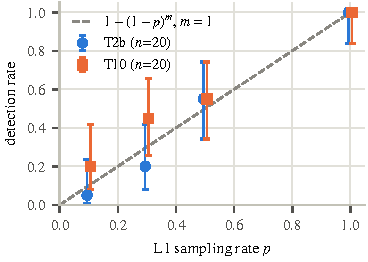
\includegraphics[width=0.75\columnwidth]{figures/fig_a1_p}
\caption{E3: detection of T2b and T10 by \Lone{} sampling rate $p$ (Wilson 95\% CI, 20 injections each) against $1-(1-p)^m$ with one falsified unit. The four $p$ values re-judge the same 20 ledger draws, so the points are nested, and $p=1$ is 20/20 by definition; false positives were measured at $p=0.3$ only.}
\label{fig:a-p}
\end{figure}


\begin{table}[h]
\centering
\caption{E3, component ablation (E3-A in the released code; recomputed from the E3 evidence without further runs): cases T1--T10 whose B4 detection rate falls when evidence components are removed (all other rates stay at their B4 values: 1, and 0.20 for T2b; T11 variants also depend on \Lone{} and the ledger). Reg.: patient registration; Accept: acceptance non-membership; Self: patient self-check; Ledger: contract transitions, cross-check, and immutability.}
\label{tab:e3a}
\footnotesize
\adjustbox{max width=\columnwidth}{%
\begin{tabular}{@{}l l@{}}
\toprule
Removed & Detection rate after removal \\
\midrule
Reg. & T1: 0 \\
Accept & -- \\
\Lone{} & T2b: 0 \\
\Ltwo{} & T6: 0 \\
\Lthree{} & T5: 0 \\
\Lfour{} & T8: 0 \\
Self & T10: 0.45 \\
Lineage & -- \\
Ledger & T9: 0 \\
Accept + Self & T2a: 0.25; T3: 0.20; T10: 0.45 \\
\Lone{} + Lineage & T2b: 0; T4: 0; T7: 0 \\
\bottomrule
\end{tabular}}
\end{table}


\emph{Concealment cases T11a--f.} Supplementary Table~\ref{S-tab:t11} compares verifiers against the six concealment variants adapted from prior work (main text, Section~\ref{M-sec:c3}); the full auditor (B4) detected all 120 instances. T11a (fine-tuning until \Lthree{} passes) passed \Lthree{} in 20/20 cases. T11b (honest retraining with the withdrawers re-injected in the last round) evaded final-model tolerance entirely, and per-round tolerance caught only 7/20 at $\varepsilon_r=10^{-2}$, the vulnerability shown by Fang et al.\ (2023). T11c (forged trajectory, Adv-F of Zhang et al.\ (2024)) was caught by every per-round verifier, but T11d (neighbor substitution, Adv-R of the same work) had zero deviation against a verifier that replays the \emph{submitted} batches even at $\varepsilon=0$ (0/20), whereas deriving batches from the committed seed rule caught it in 20/20. T11e (seed grinding) was stopped only by the configuration commitment, and T11f (unapproved program) by method approval or \Lthree{}.

\emph{E4 details.} Tables~\ref{tab:a-micro}--\ref{tab:a-l1cost} give the micro-benchmarks, the latency and bandwidth sensitivity of the multi-container deployment, and the \Lone{} sampling cost, whose detection probability sets the cost--deterrence trade-off (Table~\ref{tab:a-l1cost}).

\begin{figure}[h]
\centering
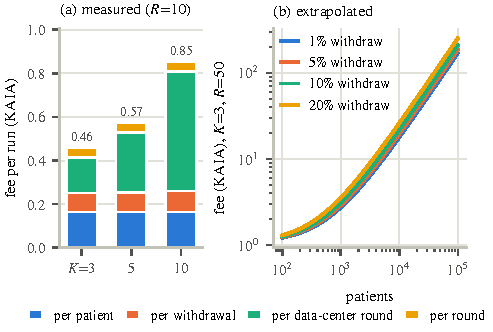
\includegraphics[width=\columnwidth]{figures/fig_e4}
\caption{E4: (a) Kairos fees per run by event type for $K=3,5,10$ (measured, 100 patients); (b) fees extrapolated from per-event costs for $K=3$ and $R=50$. Beyond about 1{,}350 patients, per-patient registration dominates at every withdrawal rate shown; raising the withdrawal rate from 1\% to 20\% raises the fee by about half (26 to 38 KAIA at 14{,}812 patients).}
\label{fig:e4}
\end{figure}

\begin{table}[h]
\centering
\caption{E4 micro-benchmarks: sorted-Merkle tree build, non-membership proof generation and verification, and proof size (JSON). Hashing the model (1.9\,MB of parameters) took 5.1\,ms and computing a binding value 1.0\,$\mu$s.}
\label{tab:a-micro}
\footnotesize
\adjustbox{max width=\columnwidth}{%
\begin{tabular}{@{}r r r r r@{}}
\toprule
Records & Build (ms) & Prove ($\mu$s) & Verify ($\mu$s) & Proof (B) \\
\midrule
100 & 0.11 & 3.3 & 8.3 & 1,216 \\
1,000 & 1.05 & 1.8 & 11.3 & 1,626 \\
10,000 & 11.09 & 3.0 & 15.7 & 2,169 \\
100,000 & 122.45 & 18.5 & 19.6 & 2,574 \\
\bottomrule
\end{tabular}}
\end{table}

\begin{table}[h]
\centering
\caption{E4 latency and bandwidth sensitivity of the multi-container deployment: mean wall-clock seconds per round ($R=10$). Delay is an artificial one-way delay applied to each request and each response; bandwidth is an artificial per-link rate. For both $K=3$ and $K=10$: one distinct final hash over the nine settings, and 3.9\,MB per round exchanged with data center 1 (the model is 1.9\,MB each way).}
\label{tab:a-lat}
\footnotesize
\adjustbox{max width=\columnwidth}{%
\begin{tabular}{@{}r r r r r@{}}
\toprule
& & \multicolumn{3}{c}{Bandwidth} \\
\cmidrule(l){3-5}
$K$ & Delay (ms) & unlimited & 100\,Mb/s & 10\,Mb/s \\
\midrule
3 & 0 & 1.92 & 2.24 & 5.02 \\
3 & 50 & 2.02 & 2.32 & 5.12 \\
3 & 200 & 2.34 & 2.64 & 5.42 \\
\midrule
10 & 0 & 2.20 & 2.44 & 5.21 \\
10 & 50 & 2.21 & 2.52 & 5.30 \\
10 & 200 & 2.52 & 2.82 & 5.61 \\
\bottomrule
\end{tabular}}
\end{table}

\begin{table}[h]
\centering
\caption{\Lone{} sampling cost (E4, $R=10$): mean re-execution time per unit, training time per round, and expected re-execution time per round, $pK\times$ unit time, for sampling rate $p$. Detection probability for $m$ falsified units is $1-(1-p)^m$; the last row gives it for $m=3$ (for $m=1$ it equals $p$).}
\label{tab:a-l1cost}
\footnotesize
\setlength{\tabcolsep}{3pt}
\adjustbox{max width=\columnwidth}{%
\begin{tabular}{@{}r r r r r r r@{}}
\toprule
& Unit & Train/round & \multicolumn{4}{c}{Re-execution per round (s) at $p$} \\
\cmidrule(l){4-7}
$K$ & (s) & (s) & 0.1 & 0.3 & 0.5 & 1.0 \\
\midrule
3 & 0.57 & 1.75 & 0.17 & 0.52 & 0.86 & 1.72 \\
5 & 0.35 & 1.79 & 0.18 & 0.53 & 0.88 & 1.76 \\
10 & 0.19 & 1.91 & 0.19 & 0.57 & 0.95 & 1.89 \\
\midrule
\multicolumn{3}{@{}l}{detection, $m=3$} & 0.27 & 0.66 & 0.88 & 1.00 \\
\bottomrule
\end{tabular}}
\end{table}


\section{Policy States and Remediation Stages}
\label{app:states}
Fig.~\ref{fig:states} shows the policy states and remediation stages of Section~\ref{M-sec:deploy} of the main text. The independent substates of each stage (pending, running, complete, failed, not applicable) are a design element; our implementation evaluates completion from recorded evidence.

\begin{figure}[h]
\centering
\adjustbox{max width=\columnwidth}{% Fig. 2: consent states (left) and the remediation stages a withdrawal activates (right).
\begin{tikzpicture}[font=\footnotesize, >=latex,
  st/.style={draw, rounded corners=6pt, align=center, inner sep=3pt, minimum width=2.3cm, minimum height=6.5mm},
  stage/.style={draw, rounded corners=2pt, align=left, inner sep=3pt, text width=4.05cm, fill=black!4},
  sub/.style={draw, rounded corners=5pt, font=\scriptsize, inner sep=2pt, minimum height=4.5mm},
  lab/.style={font=\scriptsize, align=left, inner sep=1pt}]
  % consent states
  \node[st] (none) at (0,0) {no consent};
  \node[st] (cons) at (0,-1.35) {consent $P_s^v$};
  \node[st] (req)  at (0,-2.7) {withdrawal\\[-2pt]requested};
  \node[st, very thick] (eff) at (0,-4.05) {withdrawal\\[-2pt]effective};
  \draw[->] (none) -- node[lab, right] {grant} (cons);
  \draw[->] (cons) -- node[lab, right] {$W$ on ledger\\at $\treq$} (req);
  \draw[->] (req) -- node[lab, right] {$\teff=\treq+\delta$} (eff);
  \draw[->] ([xshift=-3mm]cons.north east) arc[start angle=180, end angle=-90, radius=2.2mm] node[lab, right=2pt, pos=0.3] {change, $v{+}1$};
  \draw[->, densely dashed] (eff.west) -- ++(-0.35,0) |- node[lab, pos=0.25, left] {re-consent:\\new $v$;\\stages\\not undone} ([yshift=-1.5mm]cons.west);
  % stages
  \node[stage, anchor=north west] (s1) at (2.55,-1.0)
    {\textbf{S1} participation blocking\\[-1pt]\scriptsize level $\ge1$; non-membership at acceptance};
  \node[stage, anchor=north west] (s2) at (2.55,-2.15)
    {\textbf{S2} lineage and deployment\\[-1pt]\scriptsize level $\ge2$; revoke models from $\rzero(s)$};
  \node[stage, anchor=north west] (s3) at (2.55,-3.3)
    {\textbf{S3} influence removal\\[-1pt]\scriptsize level $3$; verified job: \Lone{}, \Ltwo{}\\[-2pt]\scriptsize (+\,\Lthree{} if approximate)};
  \coordinate (fork) at (2.15,-4.05);
  \draw[thick] (eff.east) -- (fork);
  \foreach \s in {s1,s2,s3} \draw[->, thick] (fork) |- (\s.west);
  % substates
  \node[sub] (pd) at (3.15,-4.85) {pending};
  \node[sub] (rn) at (4.45,-4.85) {running};
  \node[sub] (ok) at (5.95,-4.6) {complete};
  \node[sub] (fl) at (5.95,-5.15) {failed};
  \node[sub, dashed] (na) at (4.45,-5.35) {n/a};
  \draw[->] (pd) -- (rn); \draw[->] (rn.east) -- (ok.west); \draw[->] (rn.east) -- (fl.west);
  \node[lab, anchor=north west] at (2.55,-5.75) {substates of each stage; a stage is completed only\\by its own verification result};
\end{tikzpicture}
}
\caption{Policy states and remediation stages. An effective withdrawal activates the stages its level requires. Re-consent creates a new policy version and does not undo completed stages.}
\label{fig:states}
\end{figure}

\section{System Overview}
\label{app:overview}
Fig.~\ref{fig:overview} shows the parties of Section~\ref{M-sec:parties} of the main text and the data and control paths between them.

\begin{figure*}[t]
\centering
\adjustbox{max width=0.64\textwidth}{% Fig. 1: system overview. Solid = data and models, dashed = control and ledger records.
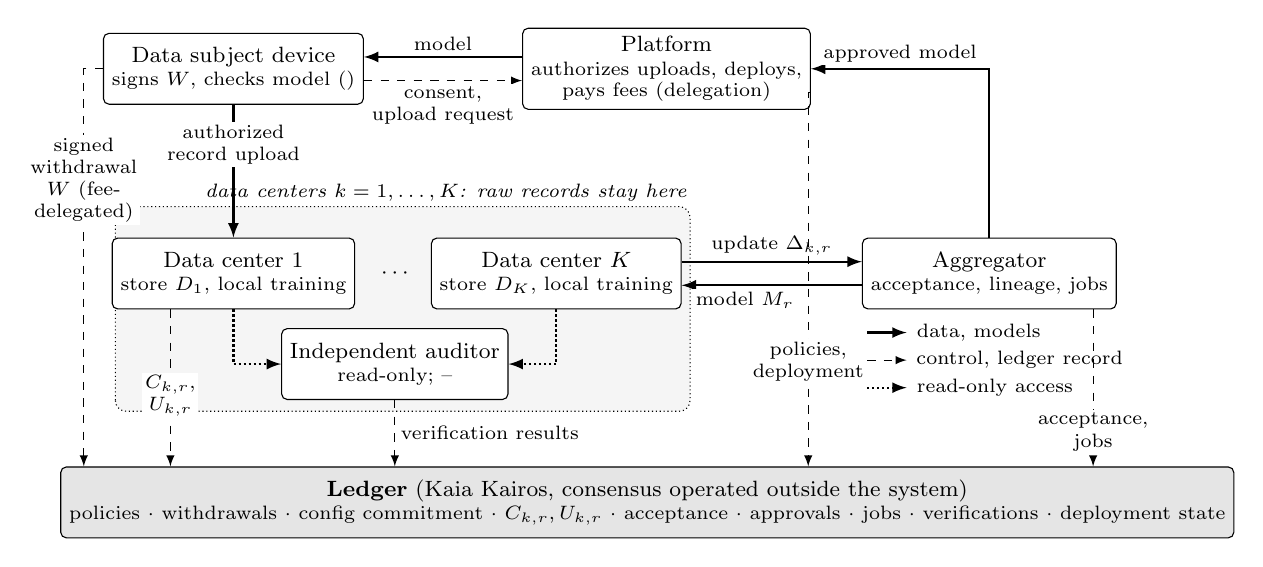
\begin{tikzpicture}[font=\footnotesize, >=latex,
  box/.style={draw, rounded corners=2pt, align=center, inner sep=3pt, minimum height=9mm, fill=white},
  data/.style={->, thick},
  ctrl/.style={->, dashed},
  lab/.style={font=\scriptsize, inner sep=1pt, fill=white, align=center}]
  % jurisdictions
  \draw[densely dotted, rounded corners=4pt, fill=black!4] (-0.9,-0.25) rectangle (6.4,2.35);
  \node[font=\scriptsize\itshape, anchor=south east, inner sep=1pt] at (6.4,2.37) {data centers $k=1,\dots,K$: raw records stay here};
  % parties
  \node[box] (dev)  at (0.6,4.1) {Data subject device\\[-1pt]\scriptsize signs $W$, checks model (\Lfour{})};
  \node[box] (plat) at (6.1,4.1) {Platform\\[-1pt]\scriptsize authorizes uploads, deploys,\\[-2pt]\scriptsize pays fees (delegation)};
  \node[box] (dc1)  at (0.6,1.5) {Data center $1$\\[-1pt]\scriptsize store $D_1$, local training};
  \node at (2.65,1.5) {$\cdots$};
  \node[box] (dck)  at (4.7,1.5) {Data center $K$\\[-1pt]\scriptsize store $D_K$, local training};
  \node[box] (aud)  at (2.65,0.35) {Independent auditor\\[-1pt]\scriptsize read-only; \Lone{}--\Lthree{}};
  \node[box] (agg)  at (10.2,1.5) {Aggregator\\[-1pt]\scriptsize acceptance, lineage, jobs};
  \node[box, minimum width=13.4cm, minimum height=9mm, fill=black!10, anchor=north west] (led) at (-1.6,-0.95)
    {\textbf{Ledger} (Kaia Kairos, consensus operated outside the system)\\[-1pt]
     \scriptsize policies $\cdot$ withdrawals $\cdot$ config commitment $\cdot$ $C_{k,r},U_{k,r}$ $\cdot$ acceptance $\cdot$ approvals $\cdot$ jobs $\cdot$ verifications $\cdot$ deployment state};
  % data path
  \draw[data] (dev.south) -- node[lab, pos=0.3] {authorized\\record upload} (dc1.north);
  \draw[data] ([yshift=1.5mm]dck.east) -- node[lab, above=1pt] {update $\Delta_{k,r}$} ([yshift=1.5mm]agg.west);
  \draw[data] ([yshift=-1.5mm]agg.west) -- node[lab, below=1pt, pos=0.65] {model $M_r$} ([yshift=-1.5mm]dck.east);
  \draw[data] (agg.north) |- node[lab, pos=0.75, above=1pt] {approved model} (plat.east);
  \draw[data] ([yshift=1.5mm]plat.west) -- node[lab, above=1pt] {model} ([yshift=1.5mm]dev.east);
  \draw[data, densely dotted] (dc1.south) |- (aud.west);
  \draw[data, densely dotted] (dck.south) |- (aud.east);
  % control path
  \draw[ctrl] ([yshift=-1.5mm]dev.east) -- node[lab, below=1pt] {consent,\\upload request} ([yshift=-1.5mm]plat.west);
  \draw[ctrl] (dev.west) -| node[lab, pos=0.64] {signed\\withdrawal\\$W$ (fee-\\delegated)} ([xshift=3mm]led.north west);
  \draw[ctrl] ([yshift=-3mm]plat.east) -| node[lab, pos=0.86] {policies,\\deployment} (7.9,-0.95);
  \draw[ctrl] ([xshift=-8mm]dc1.south) -- node[lab, pos=0.55] {$C_{k,r}$,\\$U_{k,r}$} ([xshift=-8mm]dc1.south |- led.north);
  \draw[ctrl] (aud.south) -- node[lab, right=1pt] {verification results} (aud.south |- led.north);
  \draw[ctrl] ([xshift=-3mm]agg.south east) -- node[lab, pos=0.78] {acceptance,\\jobs} ([xshift=-3mm]agg.south east |- led.north);
  % legend
  \draw[data] (8.65,0.75) -- ++(0.5,0) node[right, font=\scriptsize] {data, models};
  \draw[ctrl] (8.65,0.4) -- ++(0.5,0) node[right, font=\scriptsize] {control, ledger record};
  \draw[data, densely dotted] (8.65,0.05) -- ++(0.5,0) node[right, font=\scriptsize] {read-only access};
\end{tikzpicture}
}
\caption{System overview. Raw records never leave their data center, and the auditor reads them only inside the jurisdiction. Models travel off chain; the ledger holds commitments, decisions, and deployment state only. The platform pays the fee for the subject's withdrawal; v3.1 does not authenticate the request (Section~\ref{app:v32}).}
\label{fig:overview}
\end{figure*}

\section{Comparison with Prior Work}
\label{app:related}
Table~\ref{tab:related} compares representative work along the features targeted in the main text (Section~\ref{M-sec:related}); the references cited in it are listed at the end of this document. Until 2026-11-10 this table was Supplementary Table S1.

\begin{table*}[t]
\centering
\caption{Comparison with prior work on consent-aware learning, verifiable unlearning, and execution integrity, along the features this work targets; entries describe what each work set out to do, not whether it failed. \ding{108}~addressed, \ding{119}~partially, simulated, or conceptually, \ding{109}~not addressed, n/a: outside the work's scope (no model training); HIE: health information exchange; EMR: electronic medical records. TEE: trusted execution environment; SGX: Intel Software Guard Extensions; SNARK: succinct non-interactive argument of knowledge; MIA: membership-inference attack; PoC: proof of concept; TOST: two one-sided tests. This work: the patient self-check was simulated for the patients in the injected cases, and v3.1 does not authenticate withdrawals.}
\label{tab:related}
\scriptsize
\setlength{\tabcolsep}{2.5pt}
\renewcommand{\arraystretch}{0.9}
\newcommand{\tl}[2]{\begin{tabular}[c]{@{}l@{}}#1\\#2\end{tabular}}
\newcommand{\tc}[2]{\begin{tabular}[c]{@{}c@{}}#1\\#2\end{tabular}}
\adjustbox{max width=\textwidth}{%
\begin{tabular}{@{}l p{68pt} c c p{88pt} c p{70pt} c@{}}
\toprule
Work & \tl{Setting /}{unit} & \tc{Subject reg.\ \&}{self-check} & \tc{Decision}{time} & Execution evidence & \tc{Input}{legitimacy} & \tl{Residual test /}{approx.\ handling} & Deploy check \\
\midrule
TrustFL~\cite{zhang2020trustfl} & FL / -- & \ding{109} & \ding{109} & TEE, sampled recompute (hash) & \ding{119}~committed data & \ding{109} & \ding{109} \\
Li et al.~\cite{li2024integrity} & FL / -- & \ding{109} & \ding{109} & TEE, quantized equality replay & \ding{119}~committed data & \ding{109} & \ding{109} \\
Weng et al.~\cite{weng2024proof} & central (SISA) / sample & \ding{119}~owner checks & \ding{109} & SGX in-enclave retraining + signatures (CPU) & \ding{108}~enclave filter & \ding{109}~exact only & \ding{119}~signed predictions \\
Eisenhofer et al.~\cite{eisenhofer2025verifiable} & central / record & \ding{119}~user checks & \ding{109} & SNARK (small models, CPU) & \ding{108}~hash-chain non-membership & \ding{109}~algorithm only & \ding{109} \\
Zhuang et al.~\cite{zhuang2020patient} & HIE / patient & \ding{119}~access list & access request & n/a & n/a & n/a & n/a \\
Khan et al.~\cite{khan2025advancing} & FL / institution & \ding{109} & \ding{109} & update records & \ding{109} & \ding{109} & \ding{109} \\
Kostick-Quenet et al.~\cite{kostickquenet2025patient} & cross-silo / patient & \ding{119}~patient tracking (proposed) & training & \ding{109} & consent filter & open problem & \ding{109} \\
Fdhila et al.~\cite{fdhila2022auditable} & cross-silo / patient & \ding{119}~registration only & execution & auditor re-execution & commitments & non-retroactive & \ding{109} \\
VeriFi~\cite{gao2024verifi} & FL / participant & \ding{119}~leaver checks & \ding{119}~unlearning- enabled stage & \ding{109}~behavioral only & \ding{109} & markers, threshold $\delta$ (unspecified) & \ding{109} \\
VeriFUL~\cite{nguyen2025veriful} & FL / participant & \ding{119}~concept & \ding{109} & concept & signed request (ledger) & MIA threshold & \ding{109} \\
Zuo et al.~\cite{zuo2025blockchain} & FL (IoT) / client data & \ding{119}~client registration & \ding{109} & request/action records & \ding{119}~JWT-signed request & forgotten-class accuracy (eval.) & \ding{109} \\
Kasiraju et al.~\cite{kasiraju2025dualchain} & cross-jurisdiction / dataset & \ding{109} & periodic & lineage hashes & \ding{119}~consent docs & \ding{109} & \ding{109} \\
\textbf{This work} & \textbf{cross-silo /} \textbf{patient} & \ding{119}~simulated & \ding{108}~acceptance & \textbf{bit-exact re-exec.} \textbf{($\varepsilon=0$)} & \ding{108}~L2 & \ding{108}~TOST + pos.\ control & \ding{119}~L4 (simulated) \\
\bottomrule
\end{tabular}}
\par\smallskip\footnotesize
Ledger / evaluation: TrustFL: -- / prototype; Li et al.: -- / prototype; Weng et al.: -- / Purchase, MNIST; Eisenhofer et al.: hash chain / small tabular; Zhuang et al.: private Ethereum / simulation, tamper tests; Khan et al.: simulated chain / EMR (unnamed); Kostick-Quenet et al.: tx log / none; Fdhila et al.: permissioned (Fabric) / PoC; VeriFi: -- / image, audio; VeriFUL: permissioned / none; Zuo et al.: permissioned (Fabric) / MNIST, CIFAR-10; Kasiraju et al.: permissioned dual chain / none; this work: public testnet / fault injection.
\end{table*}

\section{Notation}
\label{app:notation}
Table~\ref{tab:notation} lists the symbols used in the main text and the Supplementary Document.

\begin{table}[h]
\centering
\caption{Notation.}
\label{tab:notation}
\footnotesize
\adjustbox{max width=\columnwidth}{%
\begin{tabular}{@{}l p{0.72\columnwidth}@{}}
\toprule
Symbol & Meaning \\
\midrule
$S_1,S_2,S_3$ & remediation stages: participation blocking, lineage and deployment management, influence removal \\
$\ell$ & remediation level in the consent policy; level $\ell$ requires $S_1,\dots,S_\ell$ \\
$P_s^v$ & consent policy of subject $s$ at version $v$: $(\tilde{s},\mathit{purpose},\mathit{scope},\mathit{valid\_from},$ $\mathit{valid\_to},\mathit{secondary},\ell,v)$ \\
$\mathit{valid}(x,t,\pi)$ & $=1$ iff, with $P_s^v$ the latest version registered by $t$: $P_s^v$ valid at $t$, $\pi\in P_s^v.\mathit{purpose}$, $x\in P_s^v.\mathit{scope}$, and $\neg\mathit{withdrawn}(s,t)$ \\
$C_{k,r}$, $U_{k,r}$ & input commitment $\mathrm{Sign}_k(k,r,\mathit{root}_S,|S|,\sigma,\pi)$ and update commitment $\mathrm{Sign}_k(k,r,\Hash(\Delta_{k,r}),h_{r-1},\Hash(C_{k,r}))$ of data center $k$ in round $r$ \\
\Lone{}--\Lfour{} & verification dimensions: execution, input, residual influence, deployment \\
$\treq,\teff,\delta$ & withdrawal request time, effective time, and delay $\teff-\treq$ \\
$\tau(k,r)$ & ledger time of the acceptance decision for data center $k$, round $r$ \\
$\rzero(s)$ & first accepted round whose input contained a record of subject $s$ \\
$J$ & remediation job: $(\mathit{jid},\tilde{s},\mathit{method},h_{\mathit{start}},$ $\{C^J_{k,r}\},\{U^J_{k,r}\},$ $h_{\mathit{out}},\prog,\mathit{seed\_rule})$ \\
$B(k,r)$, $\prog$ & binding value of a computation unit; program and environment identifier \\
$p$, $p_J$ & re-execution sampling rate for training units and job units \\
$b$, $\mathit{seed\_rule}$, $\mathit{seed}_{k,r}$ & base seed, committed derivation rule, and training seed of data center $k$ in round $r$ \\
$\eta_r$ & audit sampling seed of round $r$, drawn from the ledger after aggregation \\
$\delta_{\mathrm{L3}}$ & equivalence margin of the residual-influence test \\
A1--A12 & trust assumptions (Supplementary Table~\ref{S-tab:assumptions}) \\
E0--E4 & experiments as named in this document and the repository: E0 reproducibility and E3 withdrawal execution (main text, Section~\ref{M-sec:c3}), E1 consent-check timing (Section~\ref{M-sec:c1}), E2 unlearning and influence verification (Section~\ref{M-sec:c2}), E4 operational cost (Section~\ref{M-sec:discussion}) \\
T1--T11 & injected faults (T1--T9) and concealment cases (T10, T11) (main text, Table~\ref{M-tab:e3} and Section~\ref{M-sec:res-t11}) \\
B0--B6 & audit structures compared in E3: B0 plain cross-silo FL, B1 central consent database at selection time, B2 B1 with a signed hash-chained log, B3 B1 with a blockchain completion record (B0--B3: recording-only designs), B4 the full auditor (reference implementation), B5 the witness-co-signed log, B6 the re-execution-only auditor \\
P1, P2, U0--U5 & remediation methods compared in E2 (main text, Section~\ref{M-sec:data}): P1 blocking-only model, P2 rollback-only model, U0 retraining, U1 checkpoint replay, U2 FedEraser, U3 SISA, U4 FedOSD (U4s: larger step), U5 dropping the withdrawers' data center \\
\bottomrule
\end{tabular}}
\end{table}


\section{Ledger Events}
\label{app:events}
Table~\ref{tab:a-events} lists the contract events and the functions that emit them.

\begin{table*}[t]
\centering
\caption{ConsentLedger v3.1 events. Gas is the mean per call in the final E4 run ($K=3$); ``--'' marks calls not made in E4. With $\delta=0$, WithdrawalEffective is emitted in \textnormal{\texttt{requestWithdrawal}} (gas included); with $\delta>0$ anyone can emit it via \textnormal{\texttt{effectuate}}.}
\label{tab:a-events}
\scriptsize
\adjustbox{max width=\textwidth}{%
\begin{tabular}{@{}l l l p{0.36\textwidth} r@{}}
\toprule
Event & Function & Caller & Fields & Gas \\
\midrule
PolicyRegistered & registerPolicy & platform & subject commitment, version, policy commitment, level & 59,803 \\
WithdrawalRequested & requestWithdrawal & subject (fee-delegated) & request id, subject, version, level, record-list root & 104,757 \\
WithdrawalEffective & requestWithdrawal / effectuate & -- & request id, $\teff$ & (incl.) \\
ReceiptRootPosted & postReceiptRoot & data center & $k$, date, receipt root & -- \\
TrainingConfigCommitted & commitTrainingConfig & platform & configuration hash, time (once, before any withdrawal) & 59,679 \\
RoundOpened & openRound & platform & $r$, deadline, start model & 60,769 \\
RoundInputCommitted & commitInput & data center & $k$, $r$, $\mathit{root}_S$, $|S|$, $\sigma$, $\pi$ & 66,817 \\
UpdateCommitted & commitUpdate & data center & $k$, $r$, $\Hash(\Delta)$, $h_{\mathit{start}}$, keccak of $C$'s fields & 62,332 \\
UpdateAccepted / Rejected & decide & aggregator & $k$, $r$, $\tau$, withdrawal version / reason & 69,883 \\
RoundAggregated & aggregate & aggregator & $r$, accepted count, $h_{\mathit{out}}$, state hash & 67,079 \\
FirstUseDeclared & declareFirstUse & data center & request id, $\rzero$ & 52,535 \\
AuditSampled & sampleAudit & auditor & $r$, sampling seed, time (after aggregation) & 37,979 \\
MethodApproved & approveMethod & platform & method, $\prog$, kind (exact / approximate) & -- \\
JobCreated & createJob & aggregator & job id, method, $\prog$, $h_{\mathit{start}}$, withdrawals covered, kind & -- \\
JobCompleted & completeJob & aggregator & job id, $h_{\mathit{out}}$ & -- \\
VerificationRecorded & recordVerification & auditor & target hash, dimension (\Lone{}--\Lfour{}), result, reason & -- \\
DeploymentChanged & deploy / revoke & platform & model, state (deployed / revoked), basis & -- \\
RetentionStarted / Destroyed & retention & data center & request id, $k$ & -- \\
\bottomrule
\end{tabular}}
\end{table*}

\section{\Lthree{} Operating Characteristics}
\label{app:l3power}
The \Lthree{} equivalence test was not sized in advance (Supplementary Section~\ref{S-app:algorithms}). This section reports, post hoc and without changing the rule, which differences the main setting (margin 0.05, $z$ quantile, five references) can distinguish. The analysis plan and decision criteria of this section and of Sections~\ref{app:race} and~\ref{app:rederive} were fixed and hashed before execution (\texttt{validation/PREREG.md} in the repository); deviations, failed runs, and analyses added afterwards are listed in \texttt{validation/DEVIATIONS.md}. No model was trained and no stored result was changed.

\emph{Model.} For each scenario, reference AUCs are drawn as $N(\mu,\sigma_{\mathrm{ref}}^2)$ and the tested model's AUC as $\mu+\Delta+N(0,\sigma_T^2)$, and the rule of Algorithm~\ref{S-alg:l3} is applied with the scenario's mean stored bootstrap standard error; $\sigma_{\mathrm{ref}}$ is the standard deviation of the scenario's ten retrained models. Three readings differ in what varies: a fixed audited model ($\sigma_T=0$; the decision concerns that model), a method with the training variability of retraining ($\sigma_T=\sigma_{\mathrm{ref}}$; the primary reading, fixed in advance), and the same plus record sampling, whose paired deviation between models was estimated by re-scoring the 95 stored reference models (the tested models' per-record scores were not stored). The model was checked on the 190 U0 runs, in which $\Delta=0$ holds by construction: 145 passes were observed against 143.6 predicted (95\% prediction interval 134--152), and each of the 19 scenarios lay within its interval. The standardized U0 AUCs showed no departure from normality (Shapiro--Wilk $p=0.25$).

\emph{Findings (Table~\ref{tab:a-l3power}, Fig.~\ref{fig:a-l3power}).} At 1\% withdrawal ($|X|=167$--177) the interval half-width exceeded the margin in all 30 runs, so no model could pass, and the simulated pass probability stayed at zero with 20 references. In the other 16 scenarios a method identical to retraining passes with probability 0.54--1.00 (at least 0.80 in 15) and one at half the margin with probability 0.26--0.98. A model whose true difference equals the margin passes with probability about 0.002 when the audited model is fixed, 0.005--0.114 for a method (above the nominal 0.05 in 9 of the 16 scenarios, counted when the simulated probability exceeds 0.052, three Monte Carlo standard errors above 0.05; one further scenario lies at 0.050 and 0.052 in the two simulation runs), and 0.067--0.150 when record sampling is added (all 16), because the interval omits the tested model's own training variability; the rule's standard error was 0.64--0.95 of the standard deviation actually observed over seeds and records. The positive control detects with probability 0.8 a blocking-only residual of 0.037--0.051 AUC at 5--20\% withdrawal and of 0.076--0.086 at 1\%, and the detection frequencies predicted at the observed P1 differences agree with the observed ones. More references change little: from 5 to 20, the pass probability at $\Delta=0$ in the 5\% mid scenario rises from 0.82 to 0.88 while that at the margin stays at 0.07. Over all five-reference subsets of the ten retrained models, the reported class was retained in 92.5--96.9\% of subsets, by method; none of U4's three passes and six of U4s's 11 were retained in at least 90\% of subsets.

\begin{figure*}[t]
\centering
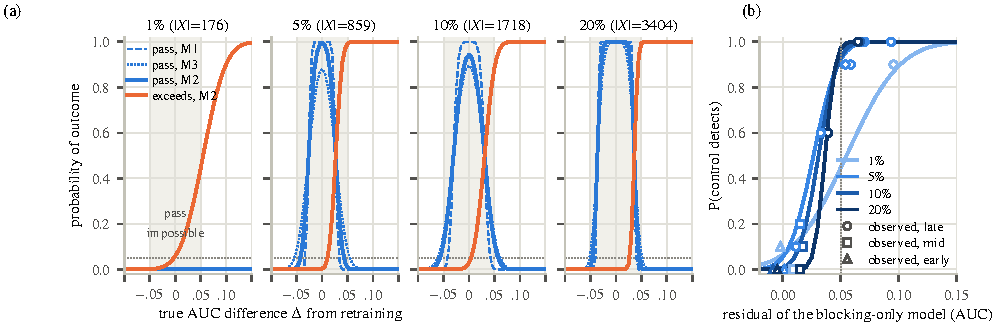
\includegraphics[width=\textwidth]{figures/fig_l3_power}
\caption{\Lthree{} operating characteristics (simulated; five references). (a) Probability of \emph{pass} and \emph{exceeds} by true difference $\Delta$ at late withdrawal of 1, 5, 10, and 20\%: M1, fixed audited model; M2, method with the training variability of retraining; M3, M2 plus record sampling. The shaded band is the margin and the dotted line the nominal 0.05. (b) Probability that the positive control detects a blocking-only residual, with the observed frequencies of P1 \emph{exceeds} in the 19 scenarios (ten seeds each) at their mean differences.}
\label{fig:a-l3power}
\end{figure*}

\begin{table*}[t]
\centering
\caption{\Lthree{} operating characteristics under the main rule (margin 0.05, $z$ quantile, five references; post hoc). $s_{\mathrm{ref}}$: standard deviation of the scenario's ten retrained models' LiRA AUC; $se_{\mathrm{boot}}$: mean stored bootstrap standard error. Simulated pass probabilities (100{,}000 draws per cell) at a true difference $\Delta$ from retraining for a fixed audited model (F; M1 in Fig.~\ref{fig:a-l3power}), a method with the training variability of retraining (M, primary; M2), and the same plus record sampling (R; M3). Residual: smallest blocking-only residual that the positive control detects with probability 0.8. P1 observed: mean difference from the reference mean, the detection probability the model predicts at that difference, and the runs classified \emph{exceeds}. U0: observed passes of retraining. Last column: P1's paired difference from retraining over the ten seeds with its 90\% $t$ interval (Table~\ref{tab:a-l3nominal}).}
\label{tab:a-l3power}
\scriptsize
\setlength{\tabcolsep}{3pt}
\adjustbox{max width=\textwidth}{%
\begin{tabular}{@{}l r c c ccc c ccc c ccc c c@{}}
\toprule
 & & & & \multicolumn{3}{c}{$P(\text{pass}\mid\Delta=0)$} & $\Delta=0.025$ & \multicolumn{3}{c}{$P(\text{pass}\mid\Delta=0.05)$} & Residual & \multicolumn{3}{c}{P1 observed} & U0 & P1 paired difference \\
\cmidrule(lr){5-7}\cmidrule(lr){8-8}\cmidrule(lr){9-11}\cmidrule(lr){13-15}
Scenario & $|X|$ & $s_{\mathrm{ref}}$ & $se_{\mathrm{boot}}$ & F & M & R & M & F & M & R & (0.8) & diff. & pred. & exceeds & pass & (90\% CI) \\
\midrule
5\%, late (base) & 859 & 0.0089 & 0.0137 & 1.000 & 0.994 & 0.881 & 0.564 & 0.000 & 0.008 & 0.085 & 0.041 & $+0.059$ & 0.98 & 9/10 & 10/10 & $+0.063$ ($+0.053$, $+0.073$) \\
1\%, late & 176 & 0.0318 & 0.0303 & 0.000 & 0.000 & 0.000 & 0.000 & 0.000 & 0.000 & 0.000 & 0.086 & $+0.096$ & 0.87 & 9/10 & 0/10 & $+0.098$ ($+0.074$, $+0.123$) \\
10\%, late & 1{,}718 & 0.0146 & 0.0099 & 1.000 & 0.942 & 0.896 & 0.635 & 0.002 & 0.114 & 0.149 & 0.042 & $+0.067$ & 1.00 & 10/10 & 10/10 & $+0.066$ ($+0.060$, $+0.072$) \\
20\%, late & 3{,}404 & 0.0051 & 0.0080 & 1.000 & 1.000 & 1.000 & 0.977 & 0.000 & 0.007 & 0.067 & 0.043 & $+0.065$ & 1.00 & 10/10 & 10/10 & $+0.065$ ($+0.060$, $+0.070$) \\
5\%, early & 840 & 0.0152 & 0.0142 & 0.999 & 0.850 & 0.723 & 0.476 & 0.000 & 0.060 & 0.119 & 0.037 & $+0.002$ & 0.02 & 0/10 & 8/10 & $+0.006$ ($-0.004$, $+0.015$) \\
5\%, mid & 851 & 0.0160 & 0.0144 & 0.998 & 0.822 & 0.702 & 0.464 & 0.000 & 0.067 & 0.125 & 0.039 & $+0.015$ & 0.22 & 2/10 & 8/10 & $+0.019$ ($+0.006$, $+0.031$) \\
1\%, early & 177 & 0.0241 & 0.0301 & 0.000 & 0.000 & 0.000 & 0.000 & 0.000 & 0.000 & 0.000 & 0.076 & $-0.002$ & 0.02 & 1/10 & 0/10 & $+0.002$ ($-0.018$, $+0.023$) \\
1\%, mid & 167 & 0.0291 & 0.0319 & 0.000 & 0.000 & 0.000 & 0.000 & 0.000 & 0.000 & 0.000 & 0.078 & $+0.009$ & 0.03 & 0/10 & 0/10 & $+0.021$ ($+0.002$, $+0.039$) \\
10\%, early & 1{,}706 & 0.0118 & 0.0101 & 1.000 & 0.983 & 0.946 & 0.687 & 0.000 & 0.076 & 0.123 & 0.043 & $-0.008$ & 0.00 & 0/10 & 10/10 & $-0.004$ ($-0.012$, $+0.004$) \\
10\%, mid & 1{,}716 & 0.0097 & 0.0098 & 1.000 & 0.998 & 0.971 & 0.753 & 0.000 & 0.050 & 0.120 & 0.040 & $+0.018$ & 0.05 & 1/10 & 10/10 & $+0.020$ ($+0.015$, $+0.025$) \\
20\%, early & 3{,}457 & 0.0093 & 0.0081 & 1.000 & 0.999 & 0.993 & 0.838 & 0.000 & 0.073 & 0.126 & 0.043 & $-0.005$ & 0.00 & 0/10 & 10/10 & $-0.005$ ($-0.011$, $+0.000$) \\
20\%, mid & 3{,}432 & 0.0077 & 0.0079 & 1.000 & 1.000 & 0.998 & 0.901 & 0.000 & 0.049 & 0.112 & 0.043 & $+0.015$ & 0.01 & 0/10 & 10/10 & $+0.015$ ($+0.008$, $+0.022$) \\
MI patients & 945 & 0.0235 & 0.0157 & 0.918 & 0.540 & 0.477 & 0.365 & 0.002 & 0.113 & 0.140 & 0.051 & $+0.093$ & 1.00 & 10/10 & 5/10 & $+0.093$ ($+0.073$, $+0.112$) \\
women aged $\ge65$ & 855 & 0.0139 & 0.0157 & 1.000 & 0.855 & 0.683 & 0.430 & 0.000 & 0.035 & 0.105 & 0.041 & $+0.071$ & 1.00 & 10/10 & 9/10 & $+0.064$ ($+0.052$, $+0.076$) \\
one institution & 850 & 0.0156 & 0.0139 & 0.999 & 0.845 & 0.732 & 0.487 & 0.000 & 0.069 & 0.125 & 0.043 & $+0.054$ & 0.92 & 9/10 & 8/10 & $+0.061$ ($+0.051$, $+0.070$) \\
three waves & 839 & 0.0097 & 0.0142 & 1.000 & 0.985 & 0.840 & 0.522 & 0.000 & 0.010 & 0.089 & 0.037 & $+0.033$ & 0.71 & 6/10 & 10/10 & $+0.035$ ($+0.027$, $+0.044$) \\
re-consent & 431 & 0.0117 & 0.0196 & 0.998 & 0.803 & 0.522 & 0.256 & 0.000 & 0.005 & 0.073 & 0.046 & $+0.011$ & 0.07 & 1/10 & 8/10 & $+0.011$ ($-0.002$, $+0.023$) \\
institution exit & 4{,}310 & 0.0143 & 0.0099 & 1.000 & 0.948 & 0.903 & 0.643 & 0.002 & 0.111 & 0.150 & 0.046 & $+0.039$ & 0.68 & 6/10 & 10/10 & $+0.048$ ($+0.041$, $+0.055$) \\
late-joining cohort & 856 & 0.0140 & 0.0139 & 1.000 & 0.894 & 0.767 & 0.499 & 0.000 & 0.052 & 0.116 & 0.037 & $+0.069$ & 1.00 & 10/10 & 9/10 & $+0.068$ ($+0.061$, $+0.075$) \\
\bottomrule
\end{tabular}}
\end{table*}


\emph{Intervals at the nominal level (Table~\ref{tab:a-l3nominal}).} After these results we applied three further interval constructions to the stored runs; this analysis is not part of the plan fixed in advance. A $t$ quantile alone leaves the boundary probability above the nominal level, by the same criterion, in 3 of the 16 scenarios (at most 0.061). Adding the references' variance for the tested model (a prediction interval) holds the level with either quantile when the method varies as retraining does (at most 0.043 and 0.017) but not when it varies more (0.104 and 0.053 at 1.5 times), and U1's AUC in the base scenario had 2.4 times the seed standard deviation of retraining. An interval that needs no such assumption uses the ten seeds of a scenario: the paired differences from retraining, the comparison for which the sample size was planned, with a $t$ interval on nine degrees of freedom. It is a statement about a method in a scenario rather than an audit decision on one model, and it is conditional on the scenario's cohort, $Z$, and shadow models. Under it, P1 is \emph{exceeds} in nine scenarios, all with late withdrawal, and in none of the eight early- and mid-withdrawal scenarios, so every pass there remains uncredited; U1, U2, and U3 are credited in 9, 7, and 9 scenarios, U4 in none, and U4s in two. The conclusions of the main text are the same under every row. The narrower scenario-level intervals (half-widths 0.004--0.028) also show what the run-level rule cannot: after mid-training withdrawal the blocking-only residual is nonzero but inside the margin ($+0.015$ to $+0.021$), so the control fails there because the residual is smaller than the margin, not because it is absent; U4s is credited at 20\% late withdrawal with a residual of $+0.044$ (90\% CI 0.039--0.050), which shows that the margin is wide relative to the blocking-only residual of about 0.065; and U2 at 1\% late withdrawal is \emph{exceeds} ($+0.038$). We keep the run-level rule, which was fixed before the reported runs, for run-level decisions; method-level conclusions rest on the scenario-level row, and the other rows are sensitivity analyses. That the qualitative conclusions agree across rows does not confer nominal error control on the run-level rule; only the prediction-interval and scenario-level constructions hold the level, each under its own assumptions.

\begin{table}[h]
\centering
\caption{\Lthree{} under intervals that approach or hold the nominal level (post hoc, added after Table~\ref{tab:a-l3power}; margin 0.05 throughout; the run-level rule is unchanged). Boundary: largest simulated probability over the scenarios that a method whose true difference equals the margin passes (nominal 0.05), when its training variability equals that of retraining ($\sigma_T=\sigma_{\mathrm{ref}}$) or is 1.5 times larger. Run level: passes over the 190 runs with the positive control applied under the same interval, and runs in which the control detected (P1 \emph{exceeds}). Scenario level: for each of the 19 scenarios, the mean of the ten seeds' paired LiRA AUC differences from retraining with a 90\% $t$ interval, classified by the same rule; passes credited only where P1 is \emph{exceeds} (without the control: U1 19, U2 16, U3 18, U4 10, U4s 12 of 19).}
\label{tab:a-l3nominal}
\footnotesize
\setlength{\tabcolsep}{3pt}
\adjustbox{max width=\columnwidth}{%
\begin{tabular}{@{}l c c c c c c c c c@{}}
\toprule
 & \multicolumn{2}{c}{Boundary} & \multicolumn{6}{c}{Passes} & P1 \\
\cmidrule(lr){2-3}\cmidrule(lr){4-9}
Interval & $\sigma_{\mathrm{ref}}$ & $1.5\,\sigma_{\mathrm{ref}}$ & U0 & U1 & U2 & U3 & U4 & U4s & exceeds \\
\midrule
\multicolumn{10}{@{}l}{\emph{Run level (of 190)}} \\
main: $s^2/n_{\mathrm{ref}}$, $z$ & 0.114 & 0.200 & 145 & 77 & 66 & 68 & 3 & 11 & 94 \\
$s^2/n_{\mathrm{ref}}$, $t$ & 0.061 & 0.135 & 122 & 61 & 51 & 54 & 2 & 8 & 88 \\
prediction: $s^2(1+1/n_{\mathrm{ref}})$, $z$ & 0.043 & 0.104 & 123 & 60 & 50 & 57 & 2 & 8 & 88 \\
prediction, $t$ & 0.017 & 0.053 & 83 & 43 & 37 & 36 & 0 & 1 & 77 \\
\midrule
\multicolumn{10}{@{}l}{\emph{Scenario level (of 19)}} \\
paired differences, $t$ (9 d.f.) & nominal & nominal & -- & 9 & 7 & 9 & 0 & 2 & 9 \\
\bottomrule
\end{tabular}}
\end{table}


\emph{Shadow-model count (Table~\ref{tab:a-shadowcount}).} The residual test used 16 shadow models per scenario. To see whether that number limits the attack, we scored each stored shadow model, whose members are handled like those of the blocking-only model, with 4, 8, or 15 of the others. After early withdrawal the AUC stayed at 0.503 for every count, and after mid-training withdrawal it rose only from 0.513 to 0.517, so within this range the missing discrimination there is unlikely to come from the number of shadow models; after late withdrawal it still rose (0.549, 0.558, 0.562), with shrinking increments. This check uses stored outputs only: it does not re-score the audited models and says nothing about counts above 16.

% Generated from results/final/shadow_count_sensitivity.json (scripts/shadow_count_sensitivity.py; stored shadow outputs only, no training).
\begin{table}[h]
\centering
\caption{Shadow-model count (post hoc). Each of the 16 stored shadow models of a scenario is scored by the offline LiRA built from $n$ of the other 15 (all 15, or the mean over 20 random subsets for $n=4$ and 8), with its own member half of the pool as members; entries are means over the 16 targets and over the scenarios of each timing (the ten late scenarios and the four early and four mid-training scenarios of the rate $\times$ timing grid). The audited models (P1, U0--U4s) are not re-scored, since their per-record statistics were not stored, and no more than 16 shadow models were trained.}
\label{tab:a-shadowcount}
\footnotesize
\setlength{\tabcolsep}{3pt}
\adjustbox{max width=\columnwidth}{%
\begin{tabular}{@{}l c c c c c c c@{}}
\toprule
 & & \multicolumn{3}{c}{AUC at $n$} & \multicolumn{3}{c}{TPR at 1\% FPR at $n$} \\
\cmidrule(lr){3-5}\cmidrule(l){6-8}
Withdrawal & Scenarios & 4 & 8 & 15 & 4 & 8 & 15 \\
\midrule
Late & 10 & 0.549 & 0.558 & 0.562 & 0.012 & 0.020 & 0.022 \\
Mid-training & 4 & 0.513 & 0.516 & 0.517 & 0.012 & 0.013 & 0.015 \\
Early & 4 & 0.503 & 0.503 & 0.503 & 0.013 & 0.012 & 0.012 \\
\bottomrule
\end{tabular}}
\end{table}


\emph{Limits.} The analysis is post hoc and rests on a normal model; record sampling is represented by differences between reference models; the ten seeds of a scenario share their references, which correlates their outcomes (intraclass correlation up to 0.11 at half the margin). It characterizes the rule and does not replace Table~\ref{tab:a-l3sens}.

\section{Acceptance Race Under Concurrent Submission}
\label{app:race}
The experiments of the main text used one sequential submitter, so the inclusion-time race (main text, Section~\ref{M-sec:race}) did not occur in them. We exercised it separately with the unmodified contract sources; the v3.1 bytecode equals the artifact used in E1--E4, and v3.2 had not run on a ledger before.

\emph{Design.} Each trial has one unit $(k,r)$, one accepting decision by the aggregator, and one withdrawal by a patient whose record is in the unit's committed input set (same hospital) or is not (other hospital). The aggregator is honest: it reads the withdrawal version, rejects if a withdrawal of the unit's hospital is visible, and otherwise accepts with the version it read. A \emph{stale acceptance} is an acceptance that succeeds although a withdrawal was ordered before it after the read; it is \emph{improper} if the withdrawer's record is in the unit. On a local EVM (py-evm, Prague) with automatic mining off, the harness fixed delivery order and block boundaries in six orderings (withdrawal confirmed before a fresh read; acceptance confirmed before the withdrawal; near-simultaneous submission; delivery order differing from submission order; same block; delayed read), each with 50 trials per contract version and hospital relation (1,200 trials), and three runs gave identical outcomes. On Kairos, both versions were newly deployed (v3.1 at \texttt{0xE24658\allowbreak be1BaC\allowbreak 5Da332\allowbreak 4FF569\allowbreak 63D379\allowbreak 1b1cBa\allowbreak 1ABE}, v3.2 at \texttt{0x8c7711\allowbreak ffECe1\allowbreak 46b486\allowbreak 792a89\allowbreak 7b0875\allowbreak 4eFA66\allowbreak 24E3}; deployed code equal to the local compilation), and two submitters on separate connections and threads sent the two transactions with offsets drawn uniformly from $\pm1.5$\,s, 150 trials per version, none excluded; inclusion order was not controlled and was classified from the receipts. Seven pilot trials on two further contracts are excluded from the analysis. The platform account paid the fees by fee delegation (about 4.3 KAIA in total: 1.81 and 2.19 for the two analysed runs and 0.26 for the pilot trials).

\emph{Results (Table~\ref{tab:a-race}).} Contract v3.1 accepted every stale read (local 259 of 259, Kairos 54 of 54; on Kairos 54 of 150 trials, Wilson 95\% CI 0.29--0.44, a rate set by the chosen offsets). In every acceptance the recorded version equaled the number of effective withdrawals at inclusion (local 550 of 550, Kairos 137 of 137), and the subject check, which uses only ledger events and the committed roots, found every improper acceptance (124 of 124 and 32 of 32) and flagged no other. Contract v3.2 produced no stale acceptance (0 of 600 and 0 of 150, Wilson 95\% upper bound 0.025): every accepting decision sent with a stale version reverted (260 of 260 with the reason \texttt{stale version} locally; 43 of 43 on Kairos, where the public endpoint returns only the failure status), and every withdrawal was recorded. An acceptance ordered before the withdrawal, in the same block or an earlier one, succeeded in every trial under both versions and was not flagged by the subject check.

\emph{Costs and limits.} Because v3.2 compares the global withdrawal version, it also reverts when the withdrawer's records are not in the unit: 127 of the 260 local reverts and 21 of the 43 on Kairos were unnecessary in this sense. One fresh read and resubmission (one transaction, no recomputation) succeeded in every case, but with unrelated withdrawals arriving in each block with probability 0.1, 0.5, and 0.9, a unit needed 1.18, 1.72, and 7.36 submissions on average, and 4 of 50 units were not accepted within 20 attempts at 0.9 (local). We count this as a cost of the fix, not as a further gap of Table~\ref{tab:gaps}. A check that compares only the event times flagged every valid acceptance that preceded a same-hospital withdrawal in the same block (local 55 of 55 and 46 of 46, Kairos 22 of 22 and 16 of 16), so an after-the-fact check must use the order within the block. On Kairos, inclusion never inverted the submission order (0 of 300), and none of 900 reads made right after a withdrawal's receipt returned stale state; the stale acceptances arose in the roughly one-second window between read and inclusion (median inclusion latency 0.8--0.9\,s). The measurement covers two submitters, one time window, and one public endpoint; the other fixes of v3.2 remain covered by local unit tests only, the four open paths are unchanged, and E1--E4 remain measurements of v3.1.

\begin{table}[h]
\centering
\caption{Acceptance race with an honest aggregator and one concurrent withdrawal per unit. Stale reads: accepting decisions sent with a version read before a withdrawal that the ledger ordered first. Stale acceptances: those that succeeded; improper: stale acceptances whose unit's committed input set held a record of the withdrawer. Unnecessary reverts: reverted although the withdrawer's records were not in the unit. Subject check: improper acceptances found from ledger events and committed roots, ordered by block, transaction index, and log index, and acceptances flagged in error. Timestamp-only check: valid same-block acceptances that precede a same-hospital withdrawal and are flagged in error when only event times are compared. Local EVM: six controlled orderings, identical outcomes in three runs. Kairos: two independent submitters, submission offsets drawn from $\pm1.5$\,s, so the counts are not incidence rates.}
\label{tab:a-race}
\footnotesize
\setlength{\tabcolsep}{3pt}
\adjustbox{max width=\columnwidth}{%
\begin{tabular}{@{}l r r r r r r c c c@{}}
\toprule
 & & Stale & \multicolumn{2}{c}{Stale acceptances} & \multicolumn{2}{c}{Reverts} & \multicolumn{2}{c}{Subject check} & Timestamp \\
\cmidrule(lr){4-5}\cmidrule(lr){6-7}\cmidrule(lr){8-9}
Run & Trials & reads & all & improper & all & unnec. & found & false & false flags \\
\midrule
Local EVM, v3.1 & 600 & 259 & 259 & 124 & 0 & -- & 124/124 & 0 & 55/55 \\
Local EVM, v3.2 & 600 & 260 & 0 & 0 & 260 & 127 & -- & 0 & 46/46 \\
Kairos, v3.1 & 150 & 54 & 54 & 32 & 0 & -- & 32/32 & 0 & 22/22 \\
Kairos, v3.2 & 150 & 43 & 0 & 0 & 43 & 21 & -- & 0 & 16/16 \\
\bottomrule
\end{tabular}}
\end{table}


\section{Independent Re-Derivation}
\label{app:rederive}
We re-derived the E3 and \Lthree{} claims with a verifier that imports none of the experiment's audit or summary code and reads four kinds of evidence: ledger events and state (read calls only), the data-split cache, stored checkpoints, and the statistics stored in the run logs. The verifier was written in the authors' environment, so this is not a third-party reproduction; what is independent is the evidence and the code.

Of 101 claims compared, 91 matched, 3 did not, and 7 could not be verified independently at the time (Table~\ref{tab:a-rederive}; row-level table in \path{validation/C_independent_audit/results/comparison.md}); one of the 7, the \Lone{} re-executions, has since been verified (below). The detection counts of Table~\ref{M-tab:e3} of the main text, T2b's 4 of 20 and its counts by sampling rate, Supplementary Tables~\ref{S-tab:t11} and~\ref{S-tab:rules}, and the 53 of 269 deployability fields were all re-derived. The type-A injection sites were recovered from the ledger and the data split alone: among 3,000 training units, the 60 whose commitment was not an honest, accepted one were exactly the injected units of T2a, T3, and T10.

\emph{Mismatches.} Both concern statements, not figures, and are corrected in the Supplementary Document. (i) An earlier version stated that every remediation job of the E3 ledger runs declared retraining; the 100 T5 jobs declared FedOSD, an approximate method, and none passed \Lthree{}, so the statement's conclusion, that the positive-control rule does not affect those runs, holds. (ii) The run logs' \Lthree{} fields for U0 were computed with the model among its own references (95 intervals; five classes differ), whereas the manuscript's counts test U0 against the other references (145 of 190); the provenance table now notes this difference.

\emph{Not independently verifiable.} That the withdrawn records were used in the 16 T2b runs whose unit was not sampled (the commitments are honest by design of the case, and the raw run folders were not kept); T5's \Lone{} and \Ltwo{} results; 95 of the 100 T6 detections, whose evidence folders were overwritten by later injections; T9b and T9c, detected by construction; and the B6 column, which follows from B6's definition.

\emph{\Lone{} re-executions, verified afterwards (2026-11-10).} The outcomes of the \Lone{} re-executions, and hence the zero false positives in 1,083 honest units, rested at the time only on the record written by the experiment's own auditor. They were then repeated by the authors, independently of the experiment's audit code and from the ledger's records: the sampled units were selected from the \texttt{AuditSampled} seeds, and the committed input roots and update hashes were taken from the ledger's events. The 206 type-B units were re-executed from the stored checkpoints in the pinned container (\path{validation/D_l1_reexec/}). For the 20 type-A runs, whose checkpoints had been deleted after the experiment, the training was regenerated deterministically without the ledger and matched the ledger round by round (start models 20 of 20, aggregated hashes 1,000 of 1,000, rejected units 20 of 20) before the 899 sampled units were re-executed (\path{validation/E_typeA_regen/}; about 40 min). All 877 honest type-A units and all 206 type-B units reproduced their committed update hashes; the 22 injected type-A units in the sample mismatched (T2a, T3, and T10 by input root, the four T2b units by output hash). Both are re-executions in the authors' environment from ledger-recorded inputs, not third-party reproductions.

\emph{Reproduction notes.} In the 10\% early scenario one record of $X$ was a member in all 16 shadow models; the run-time code gave it an undefined score that ranked first, whereas the released code guards against this, so five stored reference AUCs of that scenario are up to $5.9\times10^{-4}$ above what the released code returns (no class changes, and with the run-time scoring all 95 reference AUCs reproduce exactly). Repeating the ten seeds of that scenario with the released code, on the stored shadow and reference models, reproduced all 90 model hashes and lowered every model's AUC by 0.0002--0.0006; the differences from the references moved by less than 0.0003, and none of the 80 test outcomes changed (\texttt{scripts/compare\_c4\_rerun.py}). A comment in \texttt{fl/exp\_lira.py} stating that this case did not occur in the final rerun is incorrect; it is left in place because the experiment code is kept unchanged. For T8, 58 of the 100 delivered models now return \texttt{deployable} as true on the ledger, the ``scope after resolution'' gap of Table~\ref{tab:gaps}; T8's detection rests on the comparison with the \emph{deployed} model, not on \texttt{deployable}.

\begin{table}[h]
\centering
\caption{Independent re-derivation: claims compared, by evidence group. Match: the value re-derived from ledger events, the data split, stored checkpoints, or stored statistics, without the experiment's audit and summary code, equals the manuscript's. Not verifiable: the only evidence is a record written by the experiment's own auditor, was not preserved, or holds by construction or definition.}
\label{tab:a-rederive}
\footnotesize
\setlength{\tabcolsep}{3pt}
\adjustbox{max width=\columnwidth}{%
\begin{tabular}{@{}l r r r r@{}}
\toprule
Group & Claims & Match & Mismatch & Not verifiable \\
\midrule
E3 fault detection (main text, Table~\ref{M-tab:e3}) & 29 & 22 & 0 & 7 \\
Sampling limit of T2b and T10 & 7 & 7 & 0 & 0 \\
Concealment cases (Supplementary Table~\ref{S-tab:t11}) & 29 & 29 & 0 & 0 \\
\Lone{}--\Lfour{} verdicts & 8 & 7 & 1 & 0 \\
Positive-control rule (Supplementary Table~\ref{S-tab:rules}) & 16 & 16 & 0 & 0 \\
Deployability fields (53 of 269) & 8 & 8 & 0 & 0 \\
Provenance statements (Supplementary Section~\ref{S-app:provenance}) & 4 & 2 & 2 & 0 \\
\midrule
Total & 101 & 91 & 3 & 7 \\
\bottomrule
\end{tabular}}
\end{table}

